\chapter{Proposed Method}
\label{chap:method}

As discussed in Chapter~\ref{chap:background}, byte-level fuzzers cannot effectively test database engines because random mutations produce parser-rejected inputs that never reach deep program logic. Grammar-based fuzzers solve the syntactic validity problem but treat all SQL constructs equally, with no knowledge of which structural patterns are most likely to trigger vulnerabilities. Motivated by this observation, this chapter presents DBMS-Nautilus, a grammar-based greybox fuzzing system that combines Nautilus-style coverage-guided generation~\citep{nautilus} with a domain-specific SQL grammar engineered to target vulnerability-triggering code paths in SQLite. What makes DBMS-Nautilus different from existing fuzzers is its grammar --- the grammar determines what the fuzzer can discover; the fuzzing engine navigates within that space but cannot expand it.

Section~\ref{sec:overview} provides a high-level overview of the system and its components. Section~\ref{sec:grammar-design} presents the grammar design methodology, which constitutes the core contribution of this work. The grammar contains 520 production rules (526 with RQ1 seed rules) organized into a two-layer architecture, designed through root-cause analysis of known CVEs and guided by experimental feedback from fuzzing campaigns.

\section{System Overview}
\label{sec:overview}

DBMS-Nautilus is a grammar-based greybox fuzzer designed specifically for database engines. It combines the coverage-guided fuzzing loop of Nautilus~\citep{nautilus} with a domain-specific SQL grammar that encodes structural attack patterns associated with known vulnerability classes. Existing SQL fuzzers such as SQLsmith~\citep{sqlsmith} generate random queries against a pre-populated database, while Squirrel~\citep{squirrel} maintains an internal schema model to ensure semantic validity. DBMS-Nautilus takes a different approach: the grammar itself generates complete, self-contained SQL programs that create their own schema, populate data, and issue queries --- all starting from an empty in-memory database. This self-contained design means every test case is independently reproducible, requires no external database state, and can be replayed in isolation for crash confirmation.

The system consists of twelve components organized into a closed feedback loop, illustrated in Figure~\ref{fig:architecture}.

\begin{figure}[htbp]
\centering
\makebox[\textwidth][c]{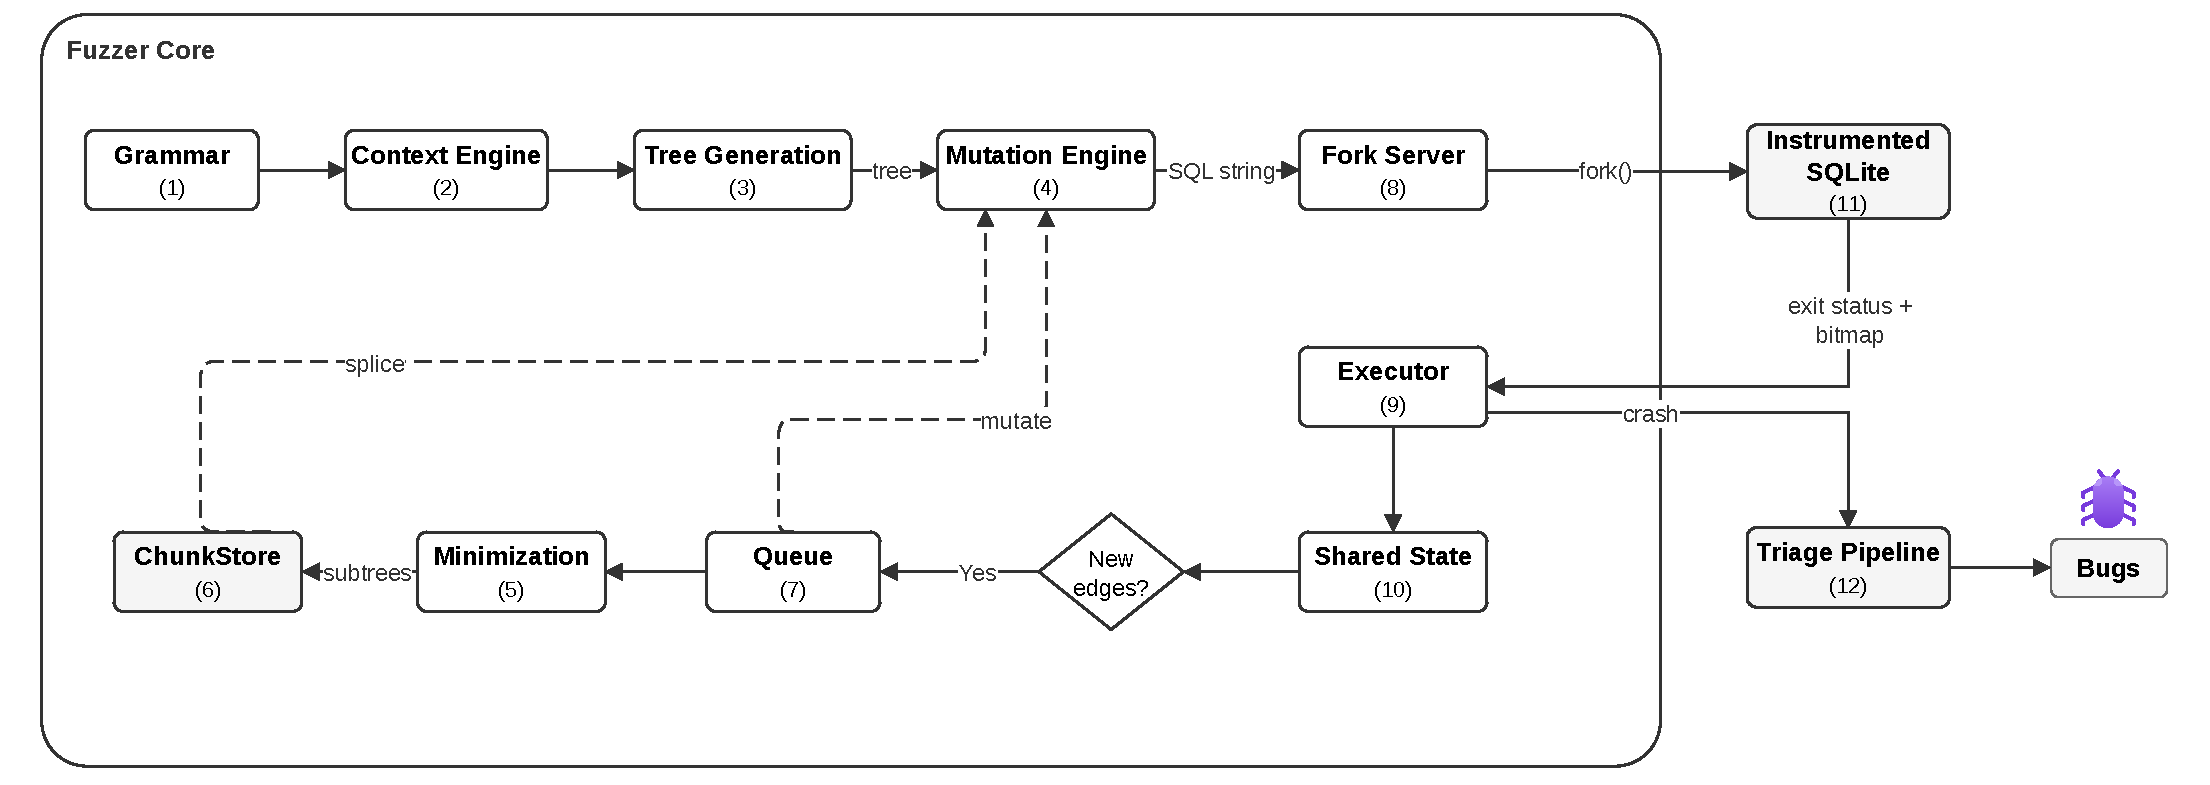
\includegraphics[width=1.25\textwidth]{figures/fig_3_1_architecture.pdf}}
\caption{Architecture of DBMS-Nautilus.}
\label{fig:architecture}
\end{figure}

Components~1 through~10 form the fuzzer core. The data flows as follows: the grammar~(1), a Python script defining 520 weighted production rules, is loaded into the context engine~(2), which stores the rules and performs weighted random selection among applicable alternatives at each non-terminal expansion. Tree generation~(3) uses the context engine to construct complete derivation trees rooted at the start symbol. These trees are either used directly (for initial seed generation) or passed through the mutation engine~(4), which applies five structural mutation operators to create variant inputs. Each mutated tree is unparsed into a SQL string and passed to the fork server~(8), which writes the SQL to a temporary file and forks a child process of the instrumented SQLite binary~(11). The child executes the SQL and exits; the fuzzer executor~(9) reads the shared memory coverage bitmap and the exit status. If the input triggered previously unseen control-flow edges, the tree is added to the queue~(7) for further mutation; if the exit indicates a crash (ASan, UBSan, or signal), the input is saved for triage. The queue manages inputs through a three-state pipeline (Init$\to$Det$\to$Random): during Init, minimization~(5) shrinks the tree while preserving its coverage contribution, and the minimized subtrees are added to the chunk store~(6) for use by splice mutations. During Det and Random, the mutation operators are applied systematically. Shared state~(10) maintains the global coverage bitmap and execution counters across all threads. After a campaign completes, the triage pipeline~(12) processes the collected crashes to deduplicate bugs and match them against known CVEs. The following sections describe each subsystem in detail.

\section{Grammar Engine}
The grammar engine defines the space of SQL inputs that the fuzzer can produce. It loads a context-free grammar specification written as a Python script, where each production rule maps a non-terminal to a string pattern containing terminal symbols and references to other non-terminals. Rules can carry numeric weights that bias the sampling distribution: at each expansion step, the engine selects among applicable rules with probability proportional to their weights, allowing the grammar designer to make certain SQL constructs more likely to appear than others. The grammar engine is the component that distinguishes DBMS-Nautilus from general-purpose grammar fuzzers: by encoding SQL-specific structural patterns and weighting them toward vulnerability-relevant constructs, it concentrates the fuzzer's effort on the most productive regions of the input space. Section~\ref{sec:grammar-design} describes the grammar design methodology in detail.

\section{Generation and Mutation}
The generation and mutation module transforms grammar rules into concrete SQL strings. On each iteration, it either builds a fresh derivation tree by expanding non-terminals according to the grammar, or takes an existing tree from the queue and applies one of five structural mutations: deterministic rule substitution (trying every alternative production at a given node), random subtree regeneration (replacing a subtree with a fresh derivation from the grammar), random recursion expansion (repeating recursive productions to increase nesting depth), splice mutation (replacing a subtree with a fragment of the same non-terminal from the chunk store), or bulk random havoc (applying repeated random subtree replacements in succession). The result is unparsed into a SQL string by reading leaf nodes left to right. This tree-level approach ensures that every generated input is syntactically valid with respect to the grammar, avoiding the wasted executions that plague byte-level mutators when applied to structured languages like SQL.

Figures~\ref{fig:mut-minimize} through~\ref{fig:mut-splice} illustrate minimization and four of the five mutation operators using SQL derivation tree examples. The fifth, bulk random havoc, applies multiple random subtree replacements in succession and is not illustrated separately.

\needspace{12\baselineskip}
In Figure~\ref{fig:mut-minimize}, the \texttt{Expr} subtree \texttt{a + b} is replaced with the smallest valid derivation of the same non-terminal (\texttt{Expr} $\to$ \texttt{Col} $\to$ \texttt{a}), producing a shorter input that preserves the same coverage bits. Subtree minimization is applied immediately after a new coverage-increasing input is discovered. The algorithm iterates over every non-terminal node in the tree and attempts to replace it with the shortest possible subtree for that non-terminal. If the replacement still triggers the same new coverage edges, the shorter tree is kept. This process reduces the tree size without losing the coverage contribution, making subsequent mutations more efficient by operating on a smaller, more focused input.
\vspace{-2mm}
\begin{figure}[H]
\centering
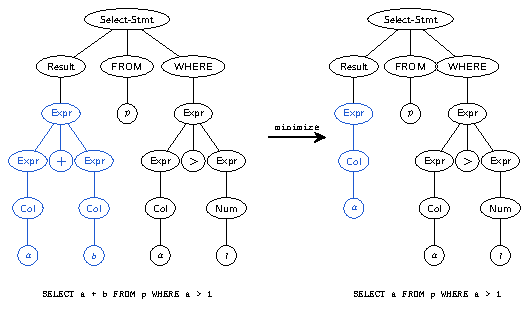
\includegraphics[width=\textwidth]{figures/mutations/fig_3_mutation_minimize.pdf}
\vspace{-3mm}
\caption{Subtree minimization.}
\label{fig:mut-minimize}
\end{figure}
\vspace{-2mm}

\needspace{12\baselineskip}
In Figure~\ref{fig:mut-rules}, the targeted \texttt{Expr} node is systematically replaced with every alternative production rule for that non-terminal, generating one mutant per rule. This deterministic mutation ensures that every possible alternative for a given non-terminal is explored at least once. For example, if \texttt{Expr} has four production rules, this operator generates four distinct mutants from a single parent tree. This exhaustive exploration is particularly valuable in the early stages of fuzzing (the Det phase), where the goal is to rapidly cover all syntactic alternatives before switching to random mutations.
\vspace{-2mm}
\begin{figure}[H]
\centering
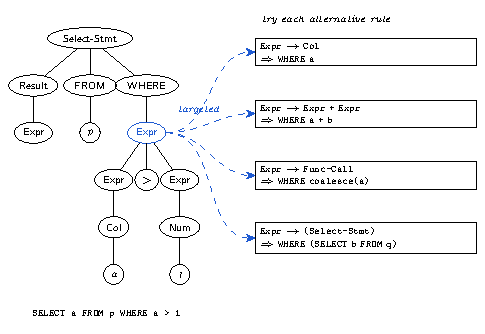
\includegraphics[width=\textwidth]{figures/mutations/fig_3_mutation_rules.pdf}
\vspace{-3mm}
\caption{Deterministic rule substitution (\texttt{mut\_rules}).}
\label{fig:mut-rules}
\end{figure}
\vspace{-2mm}

\needspace{14\baselineskip}
In Figure~\ref{fig:mut-random}, a randomly selected node's subtree is replaced with a fresh derivation from the grammar; the comparison \texttt{a > 1} is replaced with a subquery \texttt{a IN (SELECT b FROM q)}. Unlike deterministic rule substitution, which tries every alternative at a fixed node, random subtree regeneration picks both the target node and the replacement randomly. The size of the new subtree is bounded by the configured maximum tree size (set to 300 nodes in our experiments). This mutation is the primary source of structural diversity: it can introduce entirely new SQL constructs into an existing tree, such as replacing a simple comparison with a correlated subquery or a window function call.
\vspace{-2mm}
\begin{figure}[H]
\centering
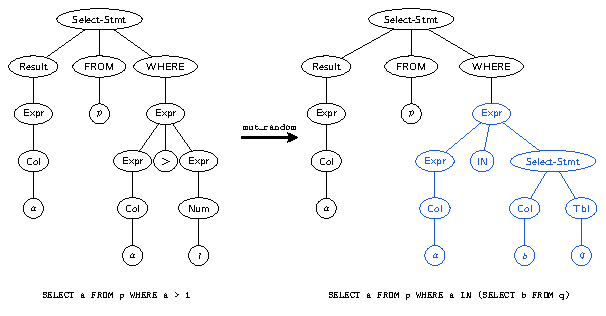
\includegraphics[width=\textwidth]{figures/mutations/fig_3_mutation_random.pdf}
\vspace{-3mm}
\caption{Random subtree regeneration (\texttt{mut\_random}).}
\label{fig:mut-random}
\end{figure}
\vspace{-2mm}

\needspace{12\baselineskip}
In Figure~\ref{fig:mut-recursion}, a recursive production (\texttt{Expr} $\to$ \texttt{Expr + Expr}) is repeated multiple times, increasing expression nesting depth. The repetition count is controlled by a randomly chosen node budget of $2 \cdot 2^k$ nodes where $k$ is chosen uniformly from $\{1, 2, \ldots, 10\}$, giving budgets from 4 to 2048; the actual number of repetitions is the budget divided by the size of the recursive structure. This mutation only expands; collapsing is performed by minimization. Deep nesting is important for vulnerability discovery because SQLite processes recursive SQL structures (nested expressions, subqueries, compound operators) through stack-based evaluation, and excessive depth can trigger stack overflows, integer overflows in intermediate computations, or null pointer dereferences when internal limits are exceeded.
\vspace{-2mm}
\begin{figure}[H]
\centering
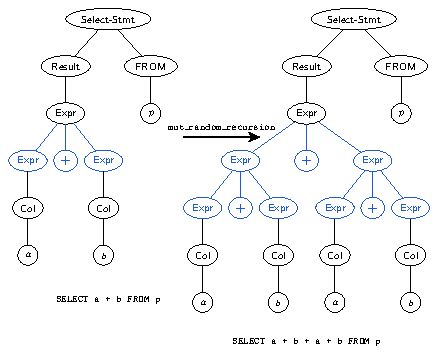
\includegraphics[width=\textwidth]{figures/mutations/fig_3_mutation_recursion.pdf}
\vspace{-3mm}
\caption{Random recursion expansion (\texttt{mut\_random\_recursion}).}
\label{fig:mut-recursion}
\end{figure}
\vspace{-2mm}

\needspace{14\baselineskip}
In Figure~\ref{fig:mut-splice}, a subtree from the ChunkStore (populated by minimized interesting inputs) replaces a compatible node in the current tree, matched by non-terminal: an \texttt{Expr} node producing \texttt{a > 1} is replaced with an \texttt{Expr} node producing \texttt{printf('\%.*g', 2147483647, 0.01)}. Splice mutation is the key mechanism for combining structural patterns discovered in separate executions. When one input discovers a new code path through a particular SQL construct, minimization extracts the relevant subtree and stores it in the ChunkStore. Splice then transplants that subtree into other inputs, creating new combinations that neither parent input could produce alone. This cross-pollination is how the fuzzer discovers bugs that require multiple structural patterns to co-occur in a single input.
\vspace{-2mm}
\begin{figure}[H]
\centering
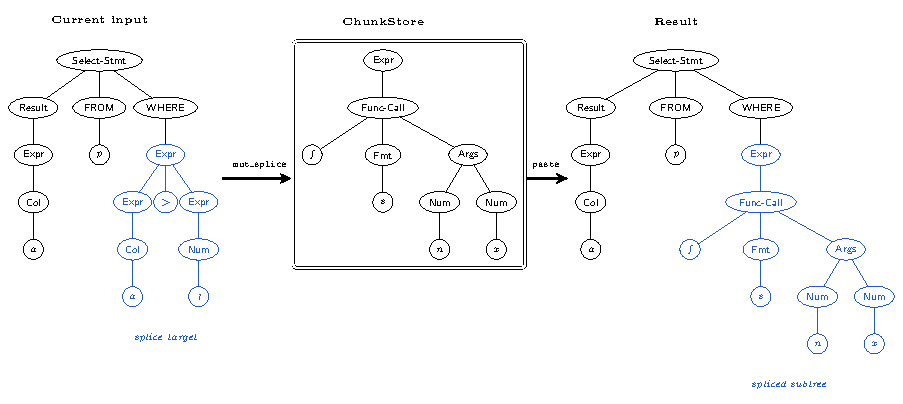
\includegraphics[width=\textwidth]{figures/mutations/fig_3_mutation_splice.pdf}
\vspace{-3mm}
\caption{Splice mutation (\texttt{mut\_splice}).}
\label{fig:mut-splice}
\end{figure}

\section{Fork Server and Harness}
The fork server and harness form the execution layer that runs each generated SQL input against a real SQLite build. The harness opens an empty in-memory SQLite database, then uses the AFL fork-server protocol~\citep{afl} to efficiently create a child process for each test case without the overhead of full process initialization. Each child executes one SQL input and exits. SQLite is compiled with AddressSanitizer (ASan) and UndefinedBehaviorSanitizer (UBSan) instrumentation, which act as oracles: ASan detects memory safety violations such as buffer overflows and use-after-free, while UBSan detects undefined behavior such as integer overflow and null pointer dereference. Without these sanitizers, many vulnerabilities would execute silently without any observable failure.

\section{Coverage Feedback and Queue}
The coverage feedback mechanism is what makes DBMS-Nautilus a \textit{greybox} fuzzer rather than a purely generative one. After each execution, the fuzzer checks whether the input exercised any previously unseen control-flow edges in SQLite by comparing the execution's coverage bitmap against the global bitmap. If new edges are found, the input is verified for deterministic behavior (re-executed five times to confirm the new edges are reproducible) and then classified as \textit{interesting} and added to the queue. The queue uses a three-state pipeline adapted from Nautilus: each input progresses through Init (minimization), Det (deterministic rule substitution plus random mutations), and Random (random mutations only). The original Nautilus uses a four-state pipeline that includes an additional \texttt{detafl} stage for AFL-style byte-level mutations; DBMS-Nautilus omits this stage because byte-level mutations (bit flips, arithmetic increments) produce parser-rejected SQL inputs that waste execution budget without reaching deep program logic. Over time, the feedback loop steers generation toward unexplored program regions, progressively expanding coverage into deeper and more complex code paths. Without coverage feedback, the fuzzer would generate inputs uniformly from the grammar with no awareness of which inputs are actually reaching new code --- a strictly less efficient strategy, as the experiments in Chapter~\ref{chap:experiments} demonstrate.

\section{Triage Pipeline}
The triage pipeline operates after a fuzzing campaign completes. It processes the collected crashing inputs to determine how many distinct bugs were found, whether any correspond to known CVEs, and how reliably each crash reproduces. This post-campaign analysis transforms raw crash data into actionable vulnerability reports. Chapter~\ref{chap:experiments} describes the triage methodology in detail.

\section{Self-Contained Test Cases}
A key design decision is that every test case begins from an empty database. The grammar generates multi-statement SQL programs that first create tables and insert data (via the \texttt{Schema-Setup} non-terminal), then issue the queries that exercise the target code paths. This contrasts with SQLsmith, which requires a pre-populated database and introspects its schema at runtime, and Squirrel, which maintains an evolving schema model during fuzzing. The self-contained approach has three advantages: the harness requires no setup beyond opening an empty database, every crashing input can be replayed in isolation without reconstructing external state, and the grammar retains full control over which schema patterns appear in each test case. Between schema creation and query execution, an \texttt{Insert-Stmt} non-terminal generates INSERT statements that populate the created tables with random rows, ensuring that subsequent queries operate on non-empty data and exercise the full execution path through SQLite's query engine. The Schema-Setup$\to$Insert-Stmt$\to$Stress-Query ordering within each generated program ensures referential consistency: tables and columns exist and contain data before they are queried. Remaining semantic errors (e.g., type mismatches in expressions) are handled gracefully by SQLite's error-tolerant execution --- they produce error return codes rather than crashes, and are thus filtered out naturally by the crash-detection oracle.

Table~\ref{tab:components} groups the twelve components into five functional subsystems, showing their implementation languages and roles in the pipeline. The components are grouped by functional subsystem with implementation sizes; components (1--12) correspond to Figure~\ref{fig:architecture}. The Grammar Spec.\ row refers to the grammar specification loaded at startup.

\begin{table}[htbp]
\caption{DBMS-Nautilus system components.}
\label{tab:components}
\centering
\footnotesize
\resizebox{\textwidth}{!}{%
\begin{tabular}{lllrl}
\toprule
\textbf{Subsystem} & \textbf{Lang.} & \textbf{Module} & \textbf{LoC} & \textbf{Key Responsibility} \\
\midrule
Grammar Spec.\ (1) & Python & \texttt{grammars/} & 840 & 520 weighted production rules \\
Context Engine (2) & Rust & \texttt{grammartec/} & \multirow{5}{*}{2{,}466} & Rule storage, weighted selection \\
Tree Generation (3) & Rust & \texttt{grammartec/} & & Derivation tree construction \\
Mutation Engine (4) & Rust & \texttt{grammartec/} & & 5 structural mutation operators \\
Minimization (5) & Rust & \texttt{grammartec/} & & Shrink trees preserving coverage \\
ChunkStore (6) & Rust & \texttt{grammartec/} & & Index subtrees ($\leq$30 nodes) for splice \\
\midrule
Queue (7) & Rust & \texttt{fuzzer/} & \multirow{3}{*}{2{,}384} & Three-state pipeline (Init$\to$Det$\to$Random) \\
Fuzzer Executor (9) & Rust & \texttt{fuzzer/} & & Per-thread coordination, dedup \\
Shared State (10) & Rust & \texttt{fuzzer/} & & Global bitmap, counters \\
\midrule
Fork Server (8) & Rust & \texttt{forksrv/} & 426 & AFL protocol, shared memory bitmap \\
Harness & C & \texttt{harness/} & 89 & Empty DB, \texttt{\_\_AFL\_INIT()}, one-exec-per-fork \\
\midrule
Triage Pipeline (12) & Python & \texttt{triage/} & 884 & Stack dedup, CVE matching, fidelity scoring \\
\bottomrule
\end{tabular}}
\end{table}


%% ====================================================================
\section{Grammar Design}
\label{sec:grammar-design}
%% ====================================================================

What makes DBMS-Nautilus different is its grammar. This grammar encodes SQL structural attack patterns that trigger vulnerability classes rather than specific proof-of-concept inputs. This ``zero PoC contamination'' principle ensures that the fuzzer discovers bugs through compositional exploration rather than replaying known attacks.

To illustrate, consider CVE-2020-9327~\citep{cve20209327}, a null pointer dereference in SQLite's generated column processor. Listing~\ref{lst:cve9327-poc} shows the original proof-of-concept from the SQLite bug tracker~\citep{cve20209327ticket}.

\begin{lstlisting}[caption={Original PoC for CVE-2020-9327.}, label={lst:cve9327-poc}, basicstyle=\ttfamily\small, numbers=none, frame=single, xleftmargin=1cm, xrightmargin=1cm]
CREATE TABLE v0(v3, v1 AS(v1) UNIQUE);
CREATE TABLE v5(v6 UNIQUE, v7 UNIQUE);
CREATE VIEW v8(v9) AS
  SELECT coalesce(v3, v1) FROM v0
  WHERE v1 IN('MED BOX');
SELECT * FROM v8 JOIN v5
  WHERE 0 > v7 AND v9 OR v6 = 's%';
\end{lstlisting}

Rather than encoding this PoC as a fixed string, the grammar decomposes it into independent, composable production rules. Table~\ref{tab:poc-decomposition} shows how each PoC element maps to a grammar rule.

\begin{table}[htbp]
\caption{Decomposition of CVE-2020-9327 PoC into grammar rules.}
\label{tab:poc-decomposition}
\centering
\scriptsize
\begin{tabular}{>{\raggedright\arraybackslash}p{2.8cm}>{\raggedright\arraybackslash}p{4.2cm}>{\raggedright\arraybackslash}p{5.8cm}}
\toprule
\textbf{\footnotesize Description} & \textbf{\footnotesize PoC SQL} & \textbf{\footnotesize Grammar Production Rule} \\
\midrule
Self-referential generated column &
  \texttt{CREATE TABLE v0(v3, v1 AS(v1) UNIQUE)} &
  \textit{Schema-Setup} $\to$ \texttt{CREATE TABLE IF NOT EXISTS p(\{Col-Def-List-GenCol\})} \newline
  \textit{Col-Def-List-GenCol} $\to$ \texttt{a \{Type-Name\}, b AS(b) UNIQUE} \\
\midrule
View wrapping the query &
  \texttt{CREATE VIEW v8(v9) AS SELECT coalesce(v3, v1) FROM v0 WHERE v1 IN('MED BOX')} &
  \textit{Schema-Setup} $\to$ \texttt{CREATE TABLE ...; CREATE VIEW IF NOT EXISTS v1 AS \{Select-Stmt\}} \\
\midrule
\texttt{coalesce()} forcing evaluation &
  \texttt{coalesce(v3, v1)} &
  \textit{Func-Call} $\to$ \texttt{coalesce(\{Expr\}, \{Expr\})} \\
\midrule
JOIN combining view with table &
  \texttt{SELECT * FROM v8 JOIN v5 WHERE 0 > v7 AND v9 OR v6 = 's\%'} &
  \textit{Stress-Query} $\to$ \texttt{SELECT \{Result-Col-List\} FROM \{Table-Name\} NATURAL JOIN \{Table-Name\} WHERE \{Expr\}} \\
\bottomrule
\end{tabular}
\end{table}

No single grammar rule produces the complete PoC. The fuzzer must independently select a schema with generated columns, a view definition, a \texttt{coalesce} expression, and a JOIN-based query --- then compose them into a single valid SQL program. The crash is only triggered when the correct combination emerges from this compositional space.

This design philosophy yields three constraints:

\begin{enumerate}[label=(\alph*)]
    \item No grammar rule may contain a complete CVE proof-of-concept as a fixed string.
    \item Every structural pattern needed to reach a target CVE must exist as a composable non-terminal.
    \item The grammar must preserve sufficient compositional freedom to discover novel combinations beyond the known CVEs.
\end{enumerate}

A natural concern is circularity: the grammar is informed by CVE root-cause analysis, and the evaluation measures CVE rediscovery. This is by design --- known CVEs serve as ground truth. The zero PoC contamination principle (constraint~a) ensures that rediscovery is not trivial: the grammar provides structural building blocks, and the fuzzer must compose them correctly from a large combinatorial space. Chapter~\ref{chap:experiments} further validates the methodology by showing that the grammar also discovers bugs beyond the known CVEs.

In its final form, the base grammar contains 520 production rules: 471 in Layer~1 (SQL atoms) and 49 in Layer~2 (composed vulnerability-targeting shapes). For the RQ1 CVE rediscovery evaluation (Chapter~\ref{chap:experiments}), six low-weight seed rules are added, bringing the total to 526. The complete grammar specification is available in the project repository as a Python script.

\subsection{Two-Layer Architecture}
\label{sec:layer-decomposition}

A SQL statement that triggers a vulnerability is never a single construct --- it is a combination of a schema definition, a query pattern, and sometimes a boundary-value function call. To capture this compositional structure, the grammar separates concerns into two layers: Layer~1 provides the vocabulary (what SQL constructs exist), and Layer~2 provides the sentences (how those constructs combine into vulnerability-triggering patterns). This separation means that adding a new SQL construct to Layer~1 automatically makes it available to all Layer~2 patterns, and adding a new Layer~2 pattern immediately benefits from all existing Layer~1 constructs.

\paragraph{Layer 1: SQL Atoms (471 rules).}
Layer~1 defines the individual SQL constructs that serve as building blocks. Table~\ref{tab:layer1-categories} groups them by category. For example, the \texttt{Expr} non-terminal has over 30 alternatives --- including arithmetic (\texttt{a + b}), comparison (\texttt{a > 1}), function calls (\texttt{coalesce(a, b)}), subqueries (\texttt{(SELECT ...)}), and window functions (\texttt{SUM(c) OVER()}). Similarly, \texttt{Col-Def} can produce a regular column (\texttt{a INTEGER}), a generated column (\texttt{b AS(b) UNIQUE}), or a column with constraints (\texttt{c TEXT NOT NULL}). Each Layer~1 rule produces a syntactically valid SQL fragment; Layer~2 composes these fragments into complete statements.

\begin{table}[htbp]
\caption{Layer~1 non-terminal categories.}
\label{tab:layer1-categories}
\centering
\small
\resizebox{\textwidth}{!}{%
\begin{tabular}{lrl}
\toprule
\textbf{Category} & \textbf{Rules} & \textbf{Examples} \\
\midrule
Expressions       & 30+ & arithmetic, comparison, subquery, window function \\
Clauses           & 20+ & SELECT, FROM, WHERE, JOIN, GROUP BY, HAVING \\
DDL statements    & 15+ & CREATE TABLE, VIEW, INDEX, TRIGGER \\
DML statements    & 10+ & INSERT, UPDATE, DELETE \\
Function calls    & 15+ & aggregate, scalar, window-specific, coalesce \\
Terminal literals  & 20+ & integers, boundary values, strings, blobs \\
Column definitions & 10+ & regular, generated (STORED/VIRTUAL), constrained \\
\bottomrule
\end{tabular}}
\end{table}

\paragraph{Layer 2: Composed Shapes (49 rules).}
Layer~2 composes Layer~1 atoms into four high-level shapes that target specific vulnerability classes. Each shape is a non-terminal whose production rules define complete SQL statement patterns. Figure~\ref{fig:two-layer} illustrates the composition hierarchy.

Every generated SQL program begins from the start symbol \texttt{Sql-Stmt}, which selects:
\begin{itemize}
    \item \texttt{Schema-Setup} (6 alternatives) --- creates the database schema. Appears in three of the four \texttt{Sql-Stmt} alternatives.
    \item \texttt{Stress-Query} (8 alternatives) --- issues a query exercising a specific code path in SQLite's query planner. Appears in two of four alternatives.
    \item \texttt{Boundary-Func-Call} (7 alternatives) --- calls a function with boundary-value arguments. Appears in one standalone alternative.
    \item \texttt{Validation-Op} (4 alternatives) --- runs a PRAGMA or consistency check. Appears in one alternative.
\end{itemize}

\noindent The required shapes appear in every generated statement. The optional shapes are selected by weighted sampling --- their probability of inclusion is controlled by their production rule weights. This means the fuzzer samples from the Cartesian product of all Layer~2 shapes: for example, a single input might combine a generated-column schema, a NATURAL JOIN query, and a \texttt{printf} boundary call, simultaneously exercising SQLite's column resolver, join optimizer, and string formatting implementation.

\begin{figure}[htbp]
\centering
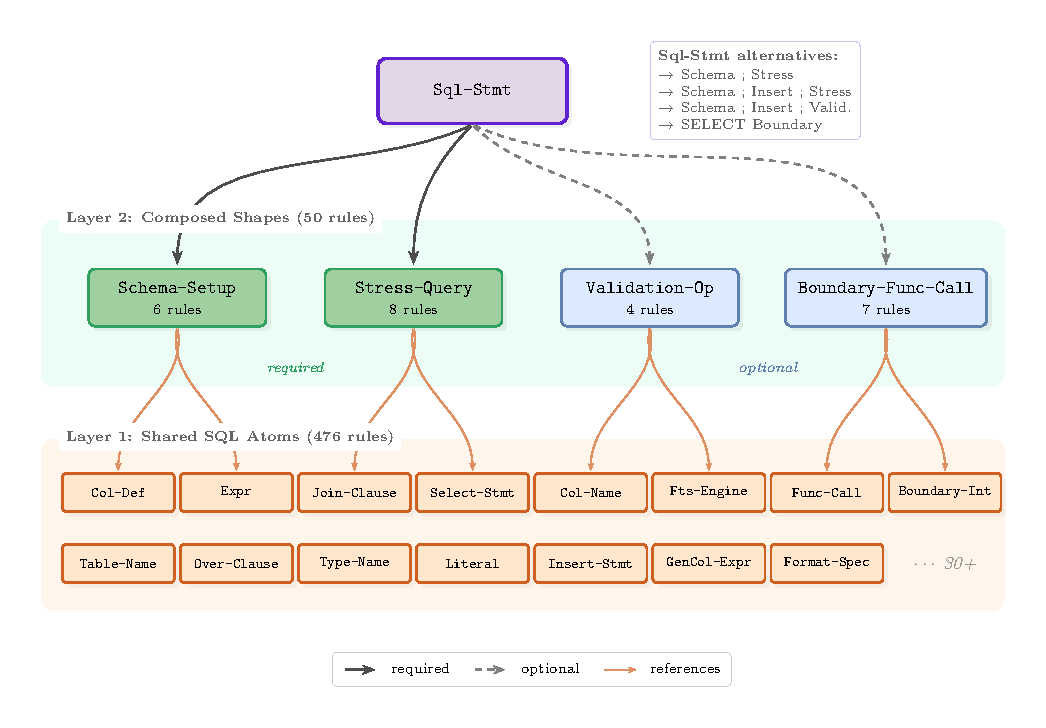
\includegraphics[width=\textwidth]{figures/fig_3_2_grammar_layers.pdf}
\caption{Two-layer grammar architecture.}
\label{fig:two-layer}
\end{figure}

\subsection{Structural Pattern Categories}
\label{sec:pattern-categories}

Each of the four Layer~2 shapes targets a distinct SQLite subsystem where vulnerabilities cluster. The categorization follows from root-cause analysis of known CVEs: each vulnerability implicates specific SQLite internals, and the grammar encodes the SQL constructs that exercise those internals. This section describes each category: what it targets, why bugs occur there, and what the grammar rules look like.

\paragraph{Schema Topology Patterns.}
The schema determines which SQLite subsystems are activated before any query runs. A simple \texttt{CREATE TABLE} only exercises the table creation code, but a schema with generated columns also activates the generated column processor, and a schema with views activates the view materializer. The \texttt{Schema-Setup} non-terminal provides six alternatives that cover these different topologies. Listing~\ref{lst:schema-setup} shows the complete set.

Why this matters: generated columns are resolved by evaluating arbitrary expressions that may reference other columns in the same table. When a column references itself --- \texttt{b AS(b) UNIQUE} --- the column resolver enters a recursive loop that can read an uninitialized pointer (CVE-2020-9327~\citep{cve20209327}) or loop infinitely (CVE-2019-19646~\citep{cve201919646}). Views add an extra layer of column resolution: the view's SELECT statement must be re-resolved every time the view is queried, creating additional opportunities for null dereferences during column name matching. The relative sampling priority of each alternative reflects how many target CVEs involve that schema shape: generated columns participate in two CVEs, while FTS virtual tables serve primarily as a diversity source.

\begin{lstlisting}[language=Python, caption={Schema-Setup alternatives (Layer 2).}, label=lst:schema-setup, basicstyle=\ttfamily\small, numbers=left]
# S1: Single table, basic columns
ctx.rule("Schema-Setup",
    "CREATE TABLE IF NOT EXISTS p({Col-Def-List})")

# S2: Table with generated column + constraints
ctx.rule("Schema-Setup",
    "CREATE TABLE IF NOT EXISTS p({Col-Def-List-GenCol})")

# S3: Two tables (enables JOINs between p and q)
ctx.rule("Schema-Setup",
    "CREATE TABLE IF NOT EXISTS p({Col-Def-List});\n"
    "CREATE TABLE IF NOT EXISTS q({Col-Def-List})")

# S4: Table + VIEW
ctx.rule("Schema-Setup",
    "CREATE TABLE IF NOT EXISTS p({Col-Def-List});\n"
    "CREATE VIEW IF NOT EXISTS v1 AS {Select-Stmt}")

# S5: Virtual table (FTS5/FTS3)
ctx.rule("Schema-Setup",
    "CREATE VIRTUAL TABLE IF NOT EXISTS fts_t1 "
    "USING {Fts-Engine}({Col-Name-List})")

# S6: Table + INDEX
ctx.rule("Schema-Setup",
    "CREATE TABLE IF NOT EXISTS p({Col-Def-List});\n"
    "CREATE INDEX IF NOT EXISTS idx1 ON p({Col-Name})")
\end{lstlisting}

\paragraph{Query Stress Patterns.}
The query determines which optimizer and execution paths are exercised after the schema is set up. SQLite's query planner performs complex AST transformations --- join reordering, subquery flattening, compound query alignment --- each involving pointer manipulation across multiple table scopes. These transformations are where null dereferences, use-after-free, and off-by-one bugs cluster. The \texttt{Stress-Query} non-terminal provides eight patterns, each targeting a different optimizer path. Table~\ref{tab:stress-query-patterns} summarizes all eight patterns and their target code paths. Listing~\ref{lst:stress-query} shows the complete set of rules.

\begin{table}[H]
\caption{Query stress patterns and their target code paths.}
\label{tab:stress-query-patterns}
\centering
\small
\begin{tabular}{llp{6.5cm}}
\toprule
\textbf{Pattern} & \textbf{SQL Construct} & \textbf{Target Code Path} \\
\midrule
Q1 & SELECT \ldots WHERE & Basic expression evaluation and filtering \\
Q2 & WHERE EXISTS (subquery) & Correlated subquery evaluation \\
Q3 & NATURAL JOIN & Column name matching across tables~\citep{cve202013435} \\
Q4 & WITH RECURSIVE & Recursive CTE expansion with termination detection \\
Q5 & INTERSECT / EXCEPT & Compound query column alignment~\citep{cve202015358, cve202013871} \\
Q6 & Self-JOIN \ldots ON & Join optimizer with aliased self-references \\
Q7 & Nested subqueries & Subquery flattening and derived table handling \\
Q8 & EXPLAIN QUERY PLAN & Plan serialization across full optimized AST \\
\bottomrule
\end{tabular}
\end{table}

For example, NATURAL JOIN (Q3) forces SQLite's column matching algorithm to pair columns across tables by name. When combined with a schema containing generated columns (from Schema Topology), this name-matching process must also resolve the generated column expression --- creating the conditions for the null dereference in CVE-2020-13435~\citep{cve202013435}. Similarly, compound queries with EXCEPT (Q5) force the optimizer to align result columns from independently optimized subqueries, stressing the column-alignment code where CVE-2020-13871~\citep{cve202013871} and CVE-2020-15358~\citep{cve202015358} were found.

\begin{lstlisting}[language=Python, caption={Stress-Query alternatives (Layer 2).}, label=lst:stress-query, basicstyle=\ttfamily\small, numbers=left]
# Q1: Base SELECT (full compositional freedom)
ctx.rule("Stress-Query", "{Select-Stmt}")

# Q2: EXISTS subquery
ctx.rule("Stress-Query",
    "SELECT {Result-Col-List} FROM {Table-Name} "
    "WHERE EXISTS ({Select-Stmt})")

# Q3: NATURAL JOIN
ctx.rule("Stress-Query",
    "SELECT {Result-Col-List} FROM {Table-Name} "
    "NATURAL JOIN {Table-Name} WHERE {Expr}")

# Q4: Recursive CTE
ctx.rule("Stress-Query",
    "WITH RECURSIVE {Cte-Def} "
    "SELECT {Result-Col-List} FROM {Table-Name}")

# Q5: Compound query (INTERSECT/EXCEPT)
ctx.rule("Stress-Query",
    "{Select-Stmt} {Compound-Op} {Select-Stmt}")

# Q6: Self-JOIN + expression
ctx.rule("Stress-Query",
    "SELECT {Result-Col-List} FROM {Table-Name} "
    "JOIN {Table-Name} {Col-Alias} ON {Expr}")

# Q7: Nested subquery chain
ctx.rule("Stress-Query",
    "SELECT {Result-Col-List} FROM "
    "(SELECT {Result-Col-List} FROM {Table-Name} "
    "WHERE {Expr}) AS sub1")

# Q8: EXPLAIN QUERY PLAN
ctx.rule("Stress-Query",
    "EXPLAIN QUERY PLAN {Select-Stmt}")
\end{lstlisting}

\paragraph{Boundary Value Patterns.}
Some SQLite vulnerabilities are triggered not by complex query structures but by specific numeric values that overflow internal integer representations. The \texttt{Boundary-Func-Call} non-terminal combines SQLite built-in functions with boundary-value arguments --- INT32\_MAX (2147483647), INT32\_MAX+1, INT32\_MIN, and INT64\_MAX --- to probe these overflow points. Listing~\ref{lst:boundary-func} shows the seven alternatives across three function families:

\begin{itemize}
    \item \textbf{printf variants} (3 rules): pair format specifiers (\texttt{\%.*g}, \texttt{\%.*f}) with boundary integers. This is how CVE-2020-13434~\citep{cve202013434} is triggered: \texttt{printf('\%.*g', 2147483647, 0.01)} causes an integer overflow in SQLite's string formatting when the width parameter equals INT32\_MAX.
    \item \textbf{substr variants} (2 rules): exercise heap buffer boundaries with boundary-value offsets and lengths, probing the substring implementation's bounds checking.
    \item \textbf{zeroblob/round} (2 rules): \texttt{hex(zeroblob(N))} stresses memory allocation with large $N$; \texttt{round} exercises float-to-int conversion edge cases.
\end{itemize}

\begin{lstlisting}[language=Python, caption={Boundary-Func-Call alternatives.}, label=lst:boundary-func, basicstyle=\ttfamily\small, numbers=left]
ctx.rule("Boundary-Func-Call",
    "printf({Format-Spec}, {Boundary-Int}, {Boundary-Float})")
ctx.rule("Boundary-Func-Call",
    "printf({Format-Spec}, {Boundary-Int})")
ctx.rule("Boundary-Func-Call",
    "printf({Printf-Fmt-Spec}, {Boundary-Int}, {Str-Literal})")
ctx.rule("Boundary-Func-Call",
    "substr({Str-Literal}, {Boundary-Int})")
ctx.rule("Boundary-Func-Call",
    "substr({Str-Literal}, {Boundary-Int}, {Boundary-Int})")
ctx.rule("Boundary-Func-Call",
    "hex(zeroblob({Boundary-Int}))")
ctx.rule("Boundary-Func-Call",
    "round({Boundary-Float}, {Boundary-Int})")

ctx.rule("Format-Spec", "'%.*g'")
ctx.rule("Format-Spec", "'%.*f'")

ctx.rule("Boundary-Int", "2147483647")    # INT32_MAX
ctx.rule("Boundary-Int", "2147483648")    # INT32_MAX+1
ctx.rule("Boundary-Int", "-2147483648")   # INT32_MIN
ctx.rule("Boundary-Int", "9223372036854775807")  # INT64_MAX
\end{lstlisting}

\paragraph{Validation Operations.}
Normal queries exercise SQLite's query planner and execution engine, but some vulnerabilities reside in separate code paths that are only activated by maintenance operations. The \texttt{Validation-Op} non-terminal provides four such operations, shown in Listing~\ref{lst:validation-op}. These operations traverse internal data structures --- B-trees, schema tables, index metadata --- using code paths that are distinct from normal query execution. When the schema contains unusual constructs such as generated columns, these traversals can encounter unexpected states: CVE-2019-19646~\citep{cve201919646} is triggered when \texttt{PRAGMA integrity\_check} encounters a generated column with a NOT NULL constraint, causing an infinite loop in the column validation logic.

\begin{lstlisting}[language=Python, caption={Validation-Op alternatives.}, label=lst:validation-op, basicstyle=\ttfamily\small, numbers=left]
ctx.rule("Validation-Op",
    "PRAGMA integrity_check")
ctx.rule("Validation-Op",
    "PRAGMA quick_check")
ctx.rule("Validation-Op",
    "ANALYZE {Table-Name}")
ctx.rule("Validation-Op",
    "EXPLAIN QUERY PLAN {Select-Stmt}")
\end{lstlisting}

Table~\ref{tab:pattern-subsystem} summarizes the mapping between pattern categories and the SQLite subsystems they exercise. Each category exercises distinct internal code paths where vulnerabilities cluster.

\begin{table}[htbp]
\caption{Structural pattern categories.}
\label{tab:pattern-subsystem}
\centering
\small
\begin{tabular}{>{\raggedright\arraybackslash}p{3.2cm} >{\raggedright\arraybackslash}p{4.0cm} >{\raggedright\arraybackslash}p{5.5cm}}
\toprule
\textbf{Pattern Category} & \textbf{Target Subsystem} & \textbf{Vulnerability Mechanism} \\
\midrule
Schema Topology (S1--S6) & Column resolver, generated column processor, view materializer & Circular dependencies, null dereferences in column resolution \\
Query Stress (Q1--Q8) & Query planner, join optimizer, compound query engine & Name resolution errors, use-after-free in AST transforms \\
Boundary Values & printf, substr, zeroblob implementations & Integer overflow, buffer overread, allocation failures \\
Validation Ops & Integrity checker, B-tree traversal, schema validator & Page cache errors, type checking failures on unusual schemas \\
\bottomrule
\end{tabular}
\end{table}

\subsection{Cross-Pollination of Structural Patterns}
\label{sec:cross-pollination}

A key property of the grammar is that structural patterns are not labeled or isolated per CVE. Each non-terminal encodes a SQL structural affordance --- a syntactic shape that participates in one or more vulnerability-triggering code paths --- without indicating which specific vulnerability it targets. This design choice ensures that the grammar captures \emph{structural categories} of vulnerabilities rather than individual instances, and it produces a cross-pollination effect: a single non-terminal serves multiple CVEs simultaneously, and a single CVE requires patterns drawn from multiple independent non-terminals.

Cross-pollination arises naturally from the independence of Layer~2 selections. On each generated input, the fuzzer independently selects a \texttt{Schema-Setup} variant, a \texttt{Stress-Query} variant, and optionally a \texttt{Boundary-Func-Call} or \texttt{Validation-Op}. Because these selections are governed by independent weighted distributions, the fuzzer samples from the Cartesian product of all Layer~2 shapes --- producing combinations that the grammar designer never explicitly planned. For example, a single generated input might combine S2 (generated columns) with Q3 (NATURAL JOIN) and a printf boundary call, exercising the intersection of SQLite's generated column processor, join optimizer, and printf implementation simultaneously.

Table~\ref{tab:cve-structural} maps each target CVE to the structural patterns required to trigger it. Every CVE requires between two and five patterns drawn from different non-terminal groups. Several key patterns are shared across multiple CVEs: generated columns participate in two CVEs, JOIN patterns serve three, and \texttt{coalesce} appears in two. This sharing means that improving the grammar's ability to reach one CVE simultaneously improves its ability to reach others --- a multiplicative benefit that would not arise if each CVE were targeted by isolated grammar rules.

\begin{table}[htbp]
\caption{Structural patterns required for each target CVE.}
\label{tab:cve-structural}
\centering
\begin{tabular}{lrl}
\toprule
\textbf{CVE} & \textbf{Patterns} & \textbf{Required Structural Elements} \\
\midrule
CVE-2019-19646 & 2 & Generated column, PRAGMA integrity\_check \\
CVE-2020-13434 & 2 & printf() call, INT32 boundary value \\
CVE-2020-9327  & 4 & Generated column, coalesce(), JOIN, CREATE VIEW \\
CVE-2020-13435 & 5 & NATURAL JOIN, coalesce(), window OVER(), \\
               &   & UNIQUE column, IN subquery \\
CVE-2020-13871 & 3 & EXCEPT, multi-column ORDER BY, scalar subquery \\
CVE-2020-15358 & 3 & CREATE VIEW with ORDER BY, INTERSECT, \\
               &   & implicit JOIN (comma-separated FROM) \\
\bottomrule
\end{tabular}
\end{table}

This cross-pollination property has two important consequences. First, any CVE rediscovery constitutes a genuine compositional achievement: the fuzzer must independently select the correct combination of non-terminals from a large combinatorial space, with each selection governed by a weighted probability distribution. Second, the grammar discovers bugs beyond its explicit design targets. The nine non-CVE bug classes reported in Chapter~\ref{chap:experiments} --- including FTS tokenizer null dereferences, float cast overflows, and window function lifecycle errors --- were found because structural patterns intended for specific CVEs also exercise adjacent code paths containing previously undocumented defects.

\subsection{Analysis of the Grammar Design Approach}
\label{sec:grammar-analysis}

The structural primitives methodology offers several advantages over alternative grammar design strategies. The cross-pollination property, described in Section~\ref{sec:cross-pollination}, means that each new structural pattern participates in combinations with all existing patterns, expanding the reachable input space combinatorially rather than additively. The zero PoC contamination principle guarantees that the grammar remains a genuine testing tool rather than a regression suite --- any vulnerability it triggers is discovered through compositional exploration, providing confidence that the methodology can find bugs that are not yet known.

The contribution of this work is methodological rather than algorithmic: while the fuzzing engine (Nautilus) is reused, the grammar design methodology --- structural pattern categories derived from CVE root-cause analysis, weighted sampling, and zero PoC contamination --- is what enables effective vulnerability discovery. The composability of the two-layer architecture simplifies grammar extension. Adding a new non-terminal to Layer~1 makes it available to all Layer~2 shapes without modifying existing rules. Adding a new Layer~2 shape creates new compositions with all existing Layer~1 atoms. This modularity means that grammar improvements are local changes with global effects, reducing the effort required to expand the grammar's reach.

An alternative to manual grammar engineering is automated grammar inference from corpora or seeds, as explored by Skyfire~\citep{skyfire} and IFuzzer~\citep{ifuzzer}. These approaches learn syntactic structure from existing inputs, eliminating the need for domain expertise. However, they cannot encode vulnerability-specific knowledge --- identifying which SQLite subsystems to stress and which structural patterns reach vulnerable code paths requires understanding that cannot be inferred from syntactic corpora alone. The manual approach trades scalability for targeting precision, which the experiments in Chapter~\ref{chap:experiments} show is the dominant factor for CVE rediscovery. While the specific grammar rules presented here are tailored to SQLite, the underlying methodology --- identify vulnerability-prone subsystems through root-cause analysis, encode structural patterns that exercise those subsystems, and assign weights proportional to vulnerability density --- is applicable to any DBMS whose internals are sufficiently documented. Applying this methodology to PostgreSQL or MySQL would require a new grammar but the same design process.

The approach has significant limitations. First, the grammar design process requires manual domain expertise. Identifying which structural patterns are associated with a vulnerability class demands understanding of both the SQL language specification and the target DBMS's internal architecture. The grammar designer must trace from a CVE's root cause to the SQL constructs that exercise the relevant code path --- an analysis that cannot be fully automated with current techniques. Second, the grammar is sensitive to weight distribution. Incorrect weights can concentrate sampling effort on a shallow region of the bug space, starving other regions of exploration budget. For example, overweighting FTS virtual table schemas in early grammar versions caused 92\% of crashes to involve FTS bugs, crowding out other vulnerability classes until the weight was reduced. Initial weights were set proportional to the number of target CVEs requiring each pattern, then adjusted based on crash diversity in pilot campaigns. This process requires empirical feedback, creating a circularity: the grammar must be run to assess its weights, but running it with poor weights wastes campaign time. Third, the grammar imposes a hard reachability ceiling: it can only discover bugs whose structural prerequisites exist as non-terminals. If a vulnerability requires a SQL construct that the grammar does not encode --- for example, an ALTER TABLE column rename or a SAVEPOINT/RELEASE transaction pattern --- no amount of campaign time or weight tuning will trigger it. The grammar defines the boundary of what the fuzzer can discover; coverage feedback can navigate within that boundary but cannot expand it.


